\subsection{Monitoraggio e Intervento}
Il sistema di controllo e intervento adottato segue il principio 
del controllo autonomo mediante l'impiego di una Neural ODE. 
Questa strategia permette di definire un sistema di Equazioni 
Differenziali Ordinarie (ODE) che descriva il sistema del mondo 
reale con le sue relazioni, e di inserire all'interno di esso in 
modo mirato una rete neurale che controlli il dosaggio delle 
contromisure \cite{B_ttcher_2022} \cite{innes2019differentiable} 
\cite{sandoval2022neural}.

Questa tecnica ha dimostrato di produrre risultati eccellenti, 
ma è fortemente influenzata dalla corretta modellazione del sistema 
sottostante e dalla selezione della funzione di costo o di controllo 
utilizzata per addestrare il modello. La sfida principale in questo 
contesto è garantire una modellazione accurata del sistema di 
partenza e una comprensione approfondita dei risultati generati 
dal controllore. Questo perché il controllore restituisce valori 
nel range $\in [0, 1]$, i quali possono risultare difficilmente 
interpretabili. Pertanto, è fondamentale definire chiaramente in 
anticipo il significato di questo intervallo di valori nel contesto 
del mondo reale.

Inizialmente, la funzione di controllo incorporata nel modello 
agente è definita come illustrato in figura \ref{fig:controller_abm}. 
È possibile notare come siano inseriti dei parametri di controllo per 
gestire l'invocazione effettiva del controllore.

Questi parametri di controllo sono principalmente associati a quando 
è necessario, dal punto di vista pratico, richiamare la funzione di 
controllo. Da un lato, servono per ridurre il numero di chiamate al 
controllore, contribuendo così a migliorare le prestazioni, e 
dall'altro lato, rendono più realistica l'idea di avere accesso a 
un sistema di controllo solo in determinati momenti temporali, 
anziché in modo continuo. Ciò riflette anche il ritardo tra la 
raccolta dei dati, la formulazione di una contromisura appropriata 
e la sua attuazione.

In seguito, vengono definite ulteriori regole di attivazione, 
questa volta legate alla prima attivazione del controllore. 
Retrospettivamente, è evidente come avere regole di prevenzione 
già attive possa essere di grande aiuto nella gestione di una pandemia. 
Tuttavia, a volte può esserci un ritardo nel riconoscere il pericolo, 
determinato dal valore di "tolerance", il quale evita l'attivazione 
del controllore fintanto che la situazione sembra rimanere al di sotto 
della soglia minima.

\begin{minipage}{\linewidth}
	\centering
	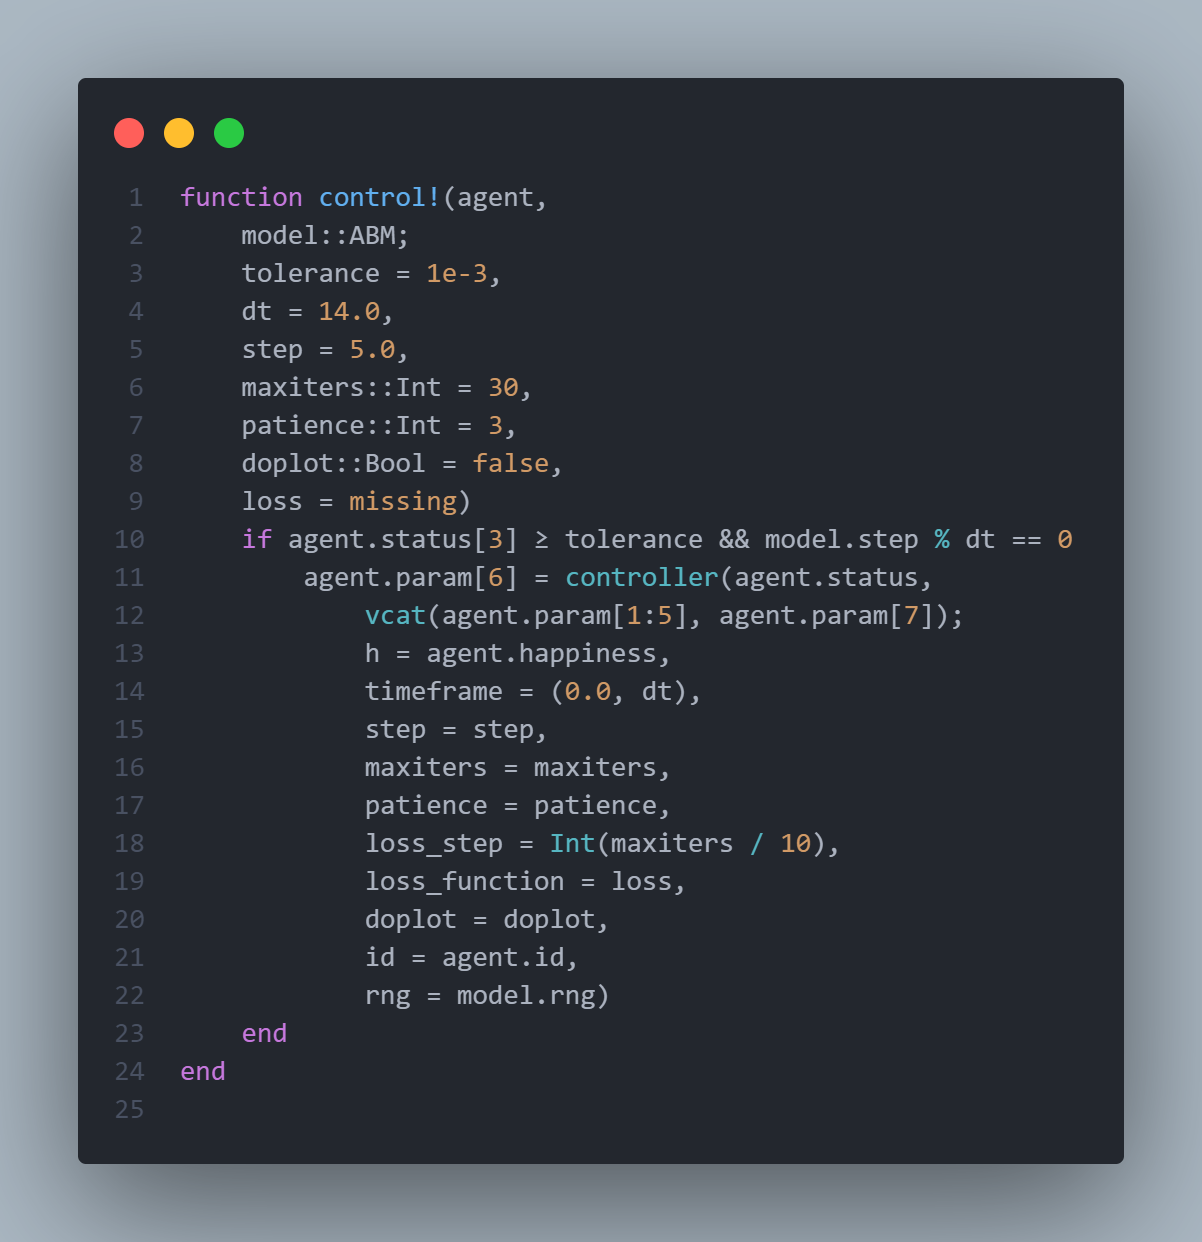
\includegraphics[width=\textwidth]{img/controller_neuralode.png}
	\captionof{figure}{Definizione del controllore all'interno del modello ad agente}
	\label{fig:controller_abm}
\end{minipage}

Altri parametri definiscono principalmente i fattori necessari affinché 
la funzione di controllo operi correttamente. 
\newpage

\subsubsection{Implementazione Controllore}

Il controllore effettivo è principalmente strutturato come già 
accennato nella sezione relativa alle Neural ODE.

Una rete neurale è definita utilizzando il framework 
\textbf{Lux.jl} \cite{pal2023lux} e viene utilizzata esclusivamente per 
fare una stima del valore di controllo $\eta$ durante la fase di 
addestramento, il quale sarà alla fine utilizzato come valore di 
controllo per il modello. Successivamente, viene definito il sistema 
di ODE che governa il fenomeno che si desidera analizzare, 
nello specifico, il sistema è un modello \textbf{SEIR} che tiene 
conto della perdita di immunità nel tempo.

\begin{minipage}{\linewidth}
	\centering
	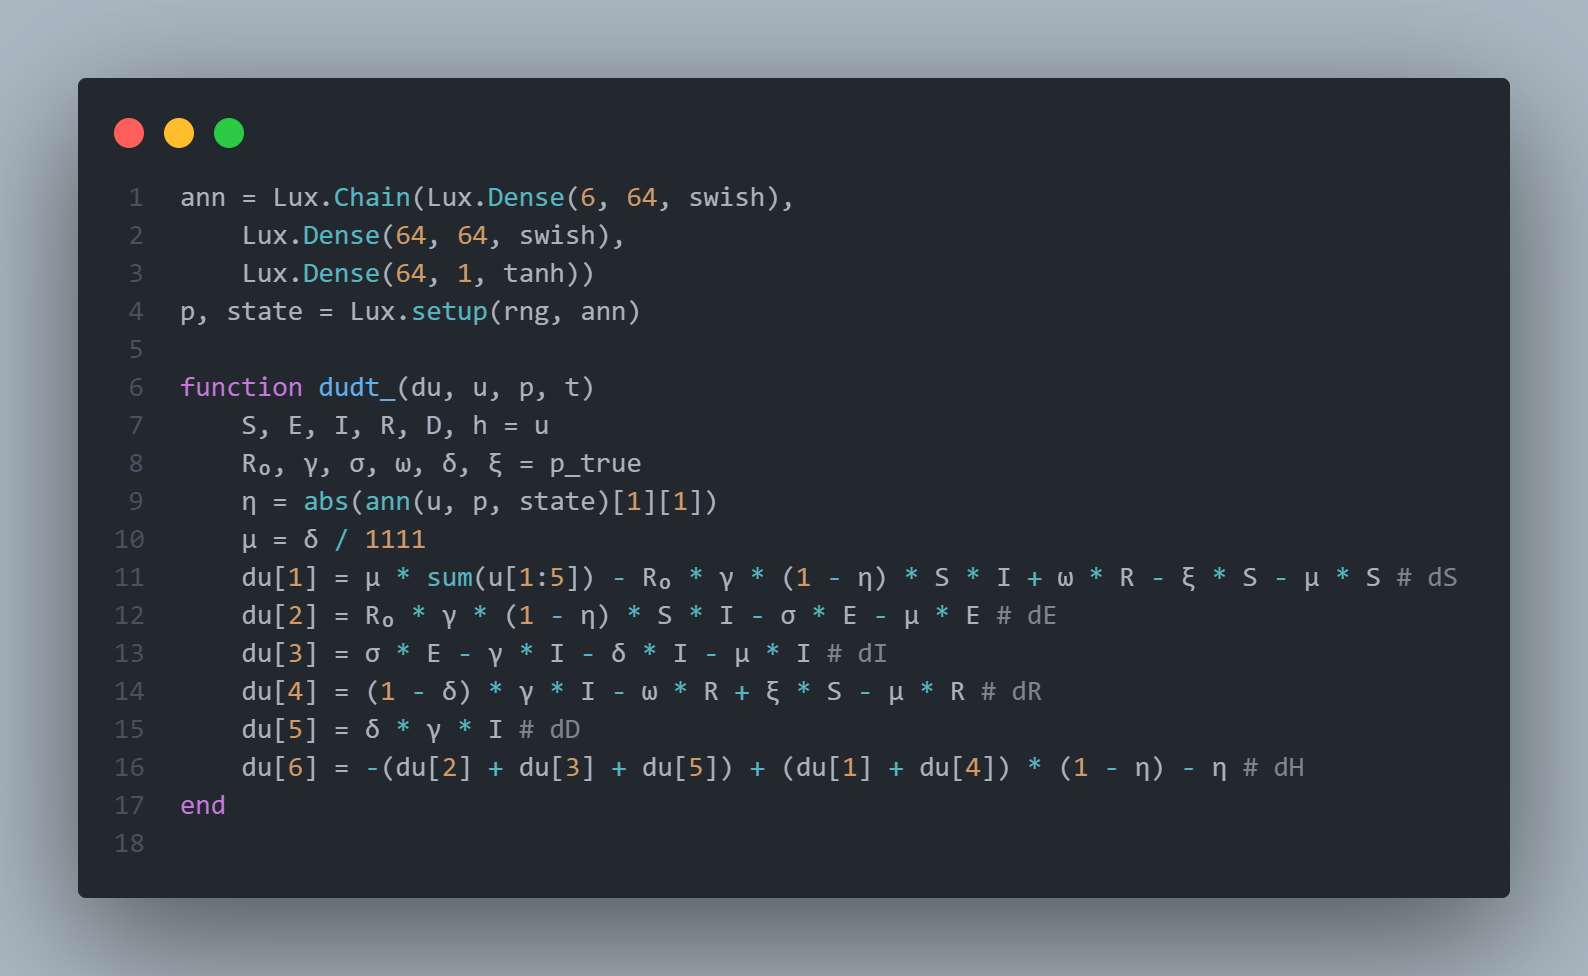
\includegraphics[width=\textwidth]{img/fann.png}
	\captionof{figure}{Definizione del controllore mediante Neural ODE}
	\label{fig:controller1}
\end{minipage}

Successivamente, il problema viene istanziato utilizzando 
l'interfaccia \textbf{ODEProblem}, a partire dalla quale il modello 
può iniziare ad essere addestrato. Prima di procedere con 
l'addestramento effettivo, vengono definite funzioni per la predizione, 
il calcolo della perdita del modello (loss) e una funzione di callback 
ausiliaria utile per monitorare l'andamento dell'apprendimento del modello.

\begin{minipage}{\linewidth}
	\centering
	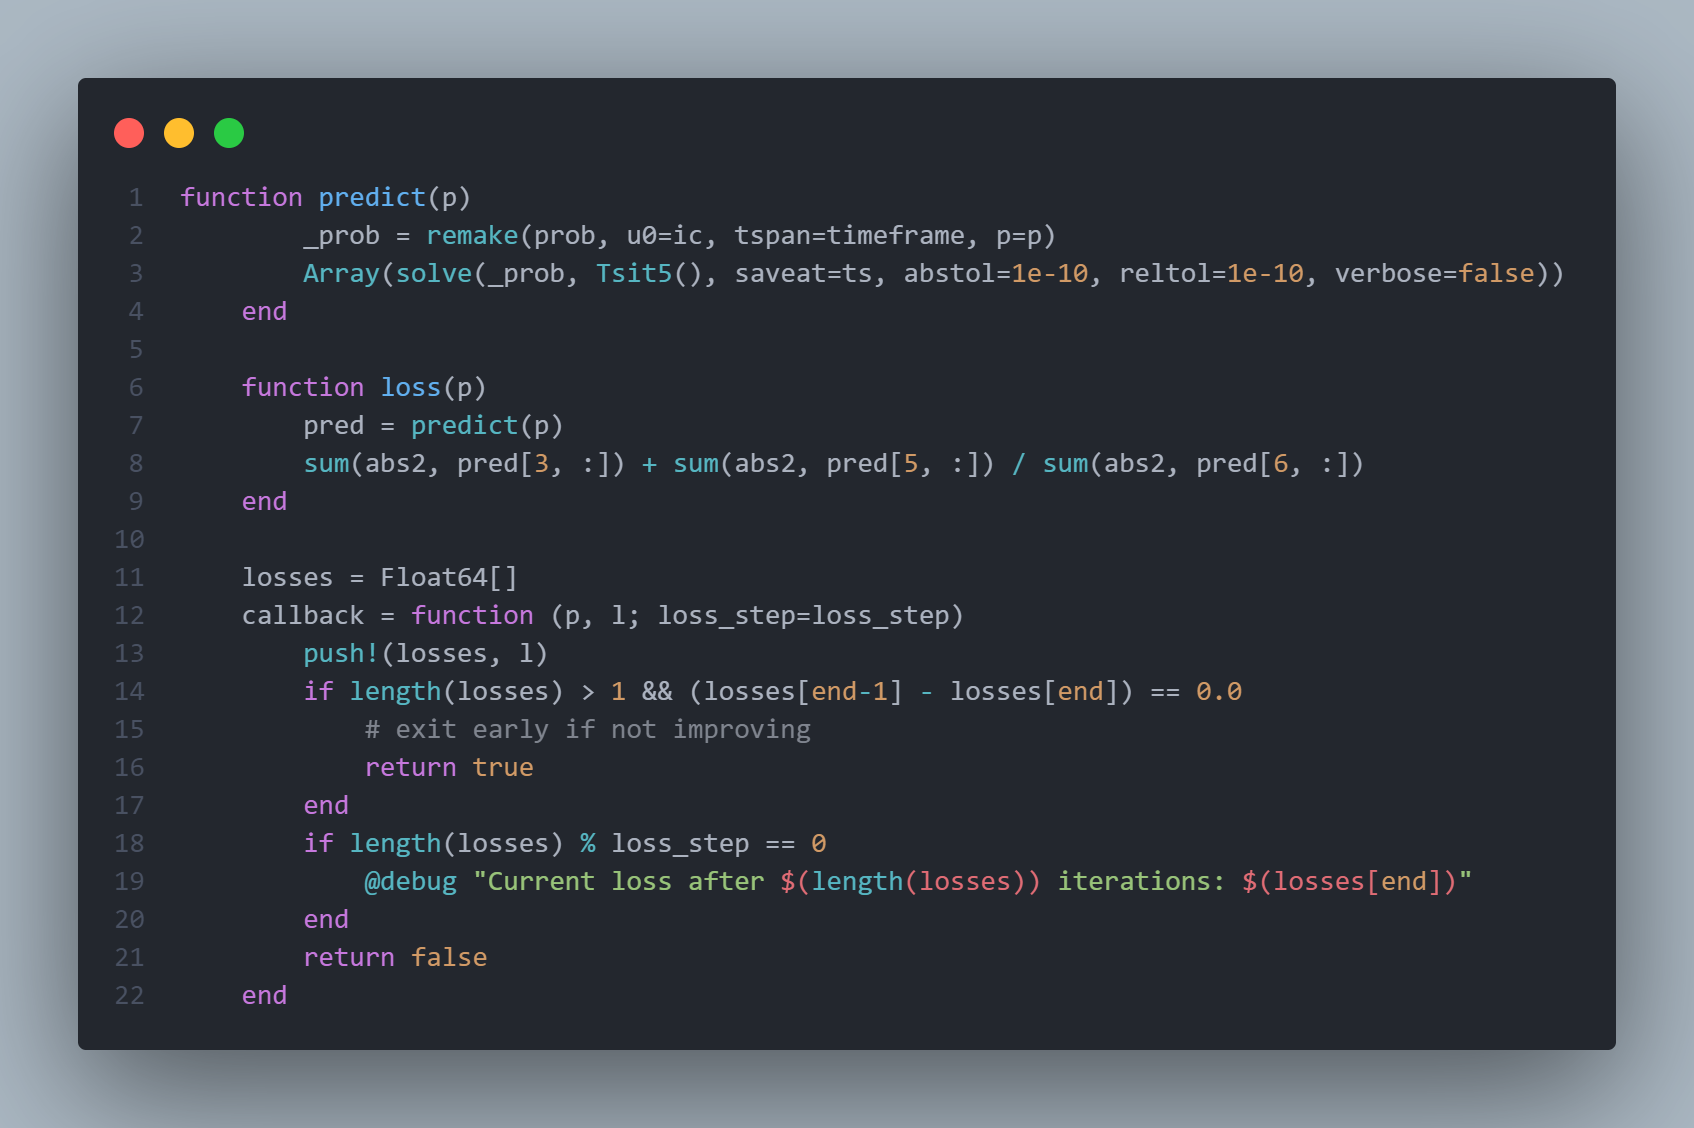
\includegraphics[width=\textwidth]{img/controller2.png}
	\captionof{figure}{Definizione delle funzioni di supporto del controllore}
	\label{fig:controller2}
\end{minipage}

Come mostrato nella figura \ref{fig:controller2}, la funzione di 
callback implementa una forma di "early stopping" per evitare 
l'addestramento eccessivo una volta che il modello ha raggiunto un 
risultato ottimale. Questo approccio si basa sull'osservazione che 
il valore della loss tende a stabilizzarsi una volta che il modello 
ha raggiunto una buona soluzione.

\newpage

\subsubsection{Esplorazione Funzione di Loss}

La definizione della funzione di perdita, come illustrato nella Figura 
\ref{fig:lossFunction}, rivela un approccio che enfatizza la 
massimizzazione del numero di individui in uno stato di salute ottimale, 
mentre cerca di minimizzare il numero di individui affetti da patologie. 
In aggiunta a questa considerazione, la funzione di perdita prende in 
considerazione il valore complessivo di felicità dell'agente, cercando di 
massimizzarlo. 

\begin{figure}[!hb]
	\centering
	\begin{subfigure}[b]{0.45\textwidth}
		\centering
		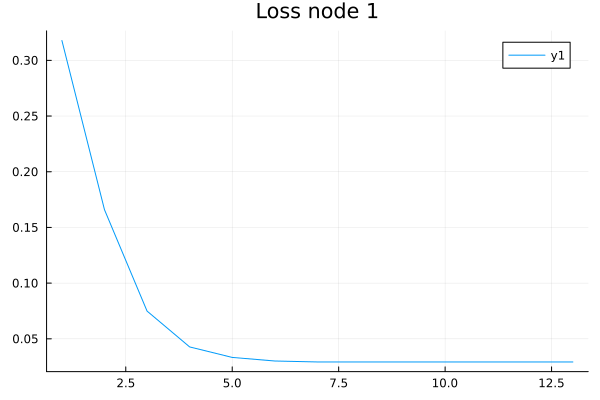
\includegraphics[width=\textwidth]{img/loss1.png}
		\caption{Esempio dell'andamento della funzione di loss durante il calcolo delle contromisure sul nodo 1}
		\label{fig:loss1}
	\end{subfigure}
	\hfill
	\begin{subfigure}[b]{0.45\textwidth}
		\centering
		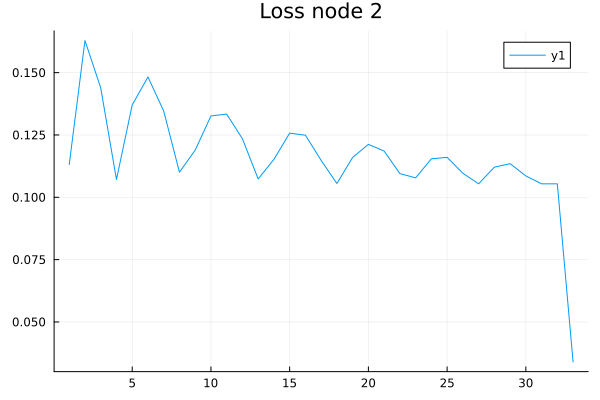
\includegraphics[width=\textwidth]{img/loss2.png}
		\caption{Esempio dell'andamento della funzione di loss durante il calcolo delle contromisure sul nodo 2}
		\label{fig:loss2}
	\end{subfigure}
	\hfill
	\begin{subfigure}[b]{0.45\textwidth}
		\centering
		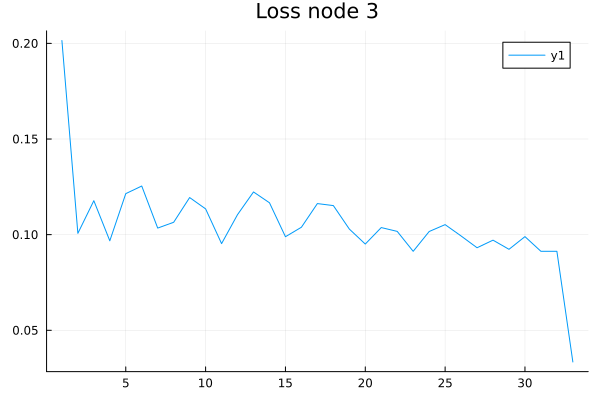
\includegraphics[width=\textwidth]{img/loss3.png}
		\caption{Esempio dell'andamento della funzione di loss durante il calcolo delle contromisure sul nodo 3}
		\label{fig:loss3}
	\end{subfigure}
	\hfill
	\begin{subfigure}[b]{0.45\textwidth}
		\centering
		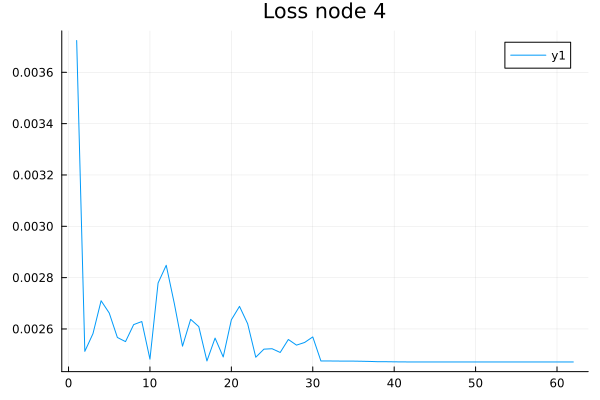
\includegraphics[width=\textwidth]{img/loss4.png}
		\caption{Esempio dell'andamento della funzione di loss durante il calcolo delle contromisure sul nodo 4}
		\label{fig:loss4}
	\end{subfigure}
\end{figure}

L'obiettivo ottimale da perseguire è rappresentato da un valore prossimo 
allo zero. È importante notare che un valore leggermente superiore a zero 
indica comunque che il modello ha identificato una soluzione accettabile, 
seppur non ottimale. Tale approccio mette in evidenza l'importanza di 
equilibrare la salute degli individui con il loro benessere complessivo, 
creando così una soluzione che tiene conto di entrambi questi aspetti 
fondamentali.

\begin{minipage}{\linewidth}
	\centering
	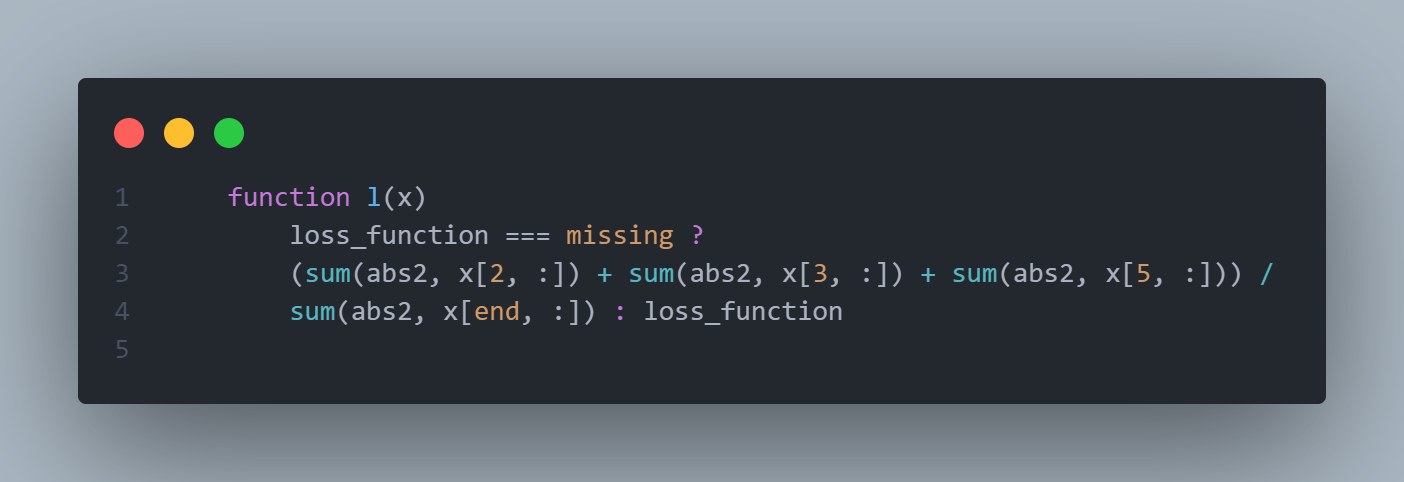
\includegraphics[width=\textwidth]{img/lossFunction.png}
	\captionof{figure}{Definizione della funzione di loss per la Rete Neurale}
	\label{fig:lossFunction}
\end{minipage}

\subsubsection{Esplorazione Funzione di Addestramento}

Il ciclo di addestramento può essere idealmente suddiviso in due parti, 
ma in pratica, entrambe potrebbero non essere necessarie. 
La prima parte, come mostrato nella figura \ref{fig:controller3}, 
impiega un ciclo di addestramento con l'uso dell'ottimizzatore 
\textbf{ADAM}. Se i risultati sono soddisfacenti, è possibile 
concludere l'addestramento. Tuttavia, è comune utilizzare due cicli 
di addestramento differenti per massimizzare le prestazioni. 
In particolare, si associano due cicli di addestramento con due 
ottimizzatori diversi al fine di sfruttare al massimo le peculiarità 
di ognuno. Questo approccio è utile per massimizzare il processo di 
ottimizzazione dei parametri. Solitamente, si utilizza un 
ottimizzatore tipo \textbf{ADAM} per la maggior parte dell'addestramento, 
in quanto è in grado di trovare rapidamente un buon spazio di iperparametri. 
Successivamente, si passa a un secondo ottimizzatore, come ad esempio 
\textbf{BFGS}, che eccelle nel trovare rapidamente un minimo locale 
all'interno dello spazio dei parametri.

Ho deciso di utilizzare un solo ottimizzatore, in quanto \textbf{ADAM} 
in questo caso, pur con un numero limitato di iterazioni, consente di 
raggiungere un risultato ottimale in tempi brevi, senza la necessità di 
utilizzare un secondo ottimizzatore, il quale in questo caso non 
apporterebbe miglioramenti significativi comportando solo un aumento 
delle risorse computazionali.

\begin{minipage}{\linewidth}
	\centering
	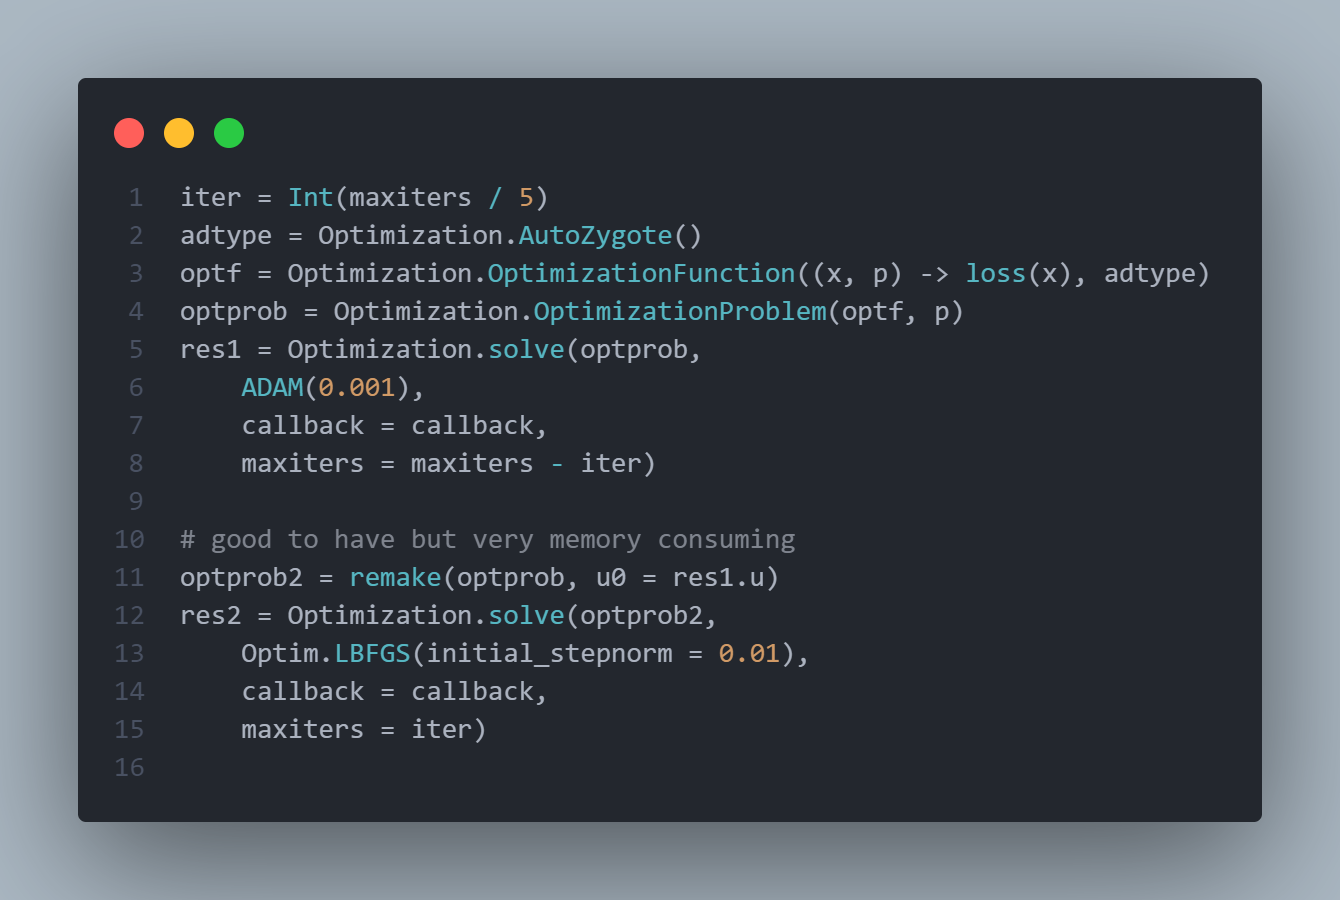
\includegraphics[width=\textwidth]{img/controller3.png}
	\captionof{figure}{Definizione delle funzioni di addestramento del controllore}
	\label{fig:controller3}
\end{minipage}

\subsubsection*{Funzione di Attivazione della Rete Neurale}
La scelta della funzione di attivazione all'interno delle reti neurali 
ha un notevole impatto sulle dinamiche di apprendimento. Attualmente, 
la funzione più comunemente utilizzata e di successo è la funzione 
\textbf{ReLU} (\textbf{Re}ctified \textbf{L}inear \textbf{U}nit), 
definita come $f(x) = \max(0, x)$. Tuttavia, sono state proposte 
diverse alternative, ma nessuna di esse è riuscita a superare la 
popolarità della ReLU, principalmente a causa di risultati 
prestazionali variabili.

La funzione di attivazione che ho scelto di utilizzare è chiamata 
\textbf{Swish} ed è stata proposta dal \emph{Google Brain Team} 
\cite{ramachandran2017searching}. La funzione Swish è definita 
come $f(x) = x \cdot sigmoid(x)$. In esperimenti condotti, è 
stato osservato che sostituire la funzione di attivazione ReLU 
con Swish ha portato a miglioramenti nelle prestazioni sui task 
di classificazione "top-1" su dataset come \textbf{ImageNet}, con 
guadagni fino al $0.9\%$ utilizzando \textbf{NASNetA} e fino al 
$0.6\%$ utilizzando \textbf{Inception-ResNet-v2}.

\begin{minipage}{\linewidth}
	\centering
	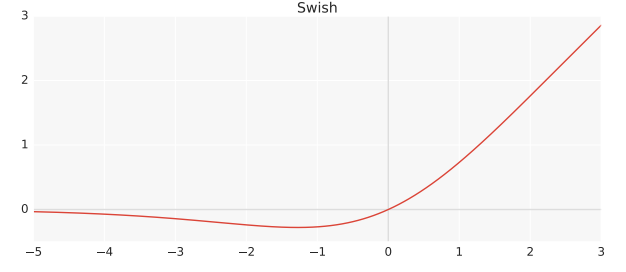
\includegraphics[width=\textwidth]{img/Screen-Shot-2017-10-18-at-2.39.55-PM.png}
	\captionof{figure}{Funzione di attivazione Swish}
	\url{https://lazyprogrammer.me/wp-content/uploads/2017/10/Screen-Shot-2017-10-18-at-2.39.55-PM.png}
	\label{fig:swish}
\end{minipage}

La peculiarità distintiva di Swish risiede nella sua semplicità e 
nella notevole somiglianza con la funzione di attivazione ReLU, 
il che la rende estremamente agevole da implementare come sua alternativa. 
Un'importante problematica associata all'utilizzo di ReLU è 
rappresentata dal fatto che il valore della sua derivata è pari 
a zero per la metà dei valori di input $x$.

È stato dimostrato, mediante l'impiego del dataset \textbf{MNIST}, 
che le prestazioni di Swish e ReLU sono sostanzialmente comparabili 
quando si utilizzano reti neurali con un numero di strati (layer) 
che si aggira intorno a 40. Tuttavia, emerge chiaramente che Swish 
supera in modo significativo ReLU in termini di prestazioni, 
specialmente quando il numero di strati si avvicina ai 40-50, 
situazione in cui l'ottimizzazione tende a diventare più complessa. 
Ciò suggerisce, ed è stato successivamente confermato, che in reti 
neurali molto profonde, Swish mostra prestazioni superiori nei test 
di accuratezza rispetto alla funzione ReLU. Tuttavia, è importante 
notare che entrambe le funzioni sperimentano un declino delle 
prestazioni all'aumentare delle dimensioni dei batch, ma in ogni caso, 
Swish ottiene risultati migliori.

Alla luce di questi dati e considerando la struttura relativamente 
poco profonda del modello, ho preso la decisione di utilizzare 
Swish come funzione di attivazione all'interno della rete neurale. 
È importante notare che questa scelta è attesa per contribuire 
positivamente alle prestazioni complessive, anche se ci si aspetta 
che il guadagno di accuratezza non sia eccessivamente sensibile, 
dato il contesto dell'applicazione illustrata nella figura 
\ref{fig:controller1}.